% !TEX TS-program = xelatex
% !BIB TS-program = bibtex
\documentclass[12pt,letterpaper]{article}
\usepackage{fontspec}
% Preserve the course style when its optional code font is unavailable.
\IfFontExistsTF{Fira Code}{}{%
  \defaultfontfeatures[Fira Code]{UprightFont=lmmono10-regular.otf}}
\usepackage{caption}
\captionsetup{font={footnotesize,it}, labelfont={bf,up}, labelsep=period,
  justification=justified, singlelinecheck=false, skip=6pt}
\usepackage{style/dsc180reportstyle}
\floatstyle{plain}
\restylefloat{table}
\usepackage{tikz}
\usetikzlibrary{positioning,arrows.meta}
\definecolor{LinkBlue}{rgb}{0.0,0.25,0.65}
% Figure palette (quarter_1_report/make_figures.py): blue subject, gray reference, warm-gray band.
\definecolor{FigBlue}{HTML}{2A78D6}
\definecolor{FigBand}{HTML}{F0EFEC}
\definecolor{FigAxis}{HTML}{C3C2B7}
\hypersetup{colorlinks=true, linkcolor=LinkBlue, citecolor=LinkBlue,
  urlcolor=LinkBlue}
\setlength{\textfloatsep}{16pt plus 2pt minus 4pt}
\setlength{\floatsep}{12pt plus 2pt minus 2pt}
\setlength{\intextsep}{14pt plus 2pt minus 4pt}
\raggedbottom
% Let text pages hold more floats, and start float-only pages at the top.
\renewcommand{\topfraction}{0.9}
\renewcommand{\bottomfraction}{0.6}
\renewcommand{\textfraction}{0.1}
\renewcommand{\floatpagefraction}{0.8}
\setcounter{topnumber}{3}
\setcounter{totalnumber}{4}
\makeatletter
\setlength{\@fptop}{0pt}
\setlength{\@fpbot}{0pt plus 1fil}
\makeatother
\widowpenalty=10000
\emergencystretch=1.5em
\clubpenalty=10000
\newcommand{\Qi}{$Q_i$}
\newcommand{\Qe}{$Q_e$}
\newcommand{\Ge}{$\Gamma_e$}

\title{Fast Neural Network Surrogates for Fusion Reactor Turbulence Simulations:\\Accuracy, Error Bars, and Transfer Between DIII-D Plasmas}
\author{Ryan Lindberg \And
  Sweekrit Bhatnagar \And
  Joseph Calderon \And
  Aryan Nath \AND
  {\normalfont Mentors: Emily Belli, Jeff Candy, and Igor Sfiligoi}}

\begin{document}
\maketitle

\begin{abstract}
  The trapped gyro-Landau fluid model TGLF predicts turbulent heat and particle fluxes in
  tokamak plasmas, but a transport simulation calls it many times. We trained neural
  network surrogates for the ion heat, electron heat, and electron particle fluxes and
  tested them in stages that move from a generic parameter scan toward real DIII-D
  plasmas. On the 5,000-case generic scan, a five-network ensemble reached test $R^2$ of
  0.958, 0.965, and 0.975 against TGLF. The same model overpredicted the particle flux of a
  DIII-D plasma by a factor of 2.1, and 67\% of the DIII-D database we then built lies
  outside the scan's ranges. Trained on 7,331 runs for DIII-D shot 128913, separate
  ensembles for each flux lowered test error by 7--22\% relative to a single joint
  ensemble, and calibrated 90\% intervals covered 91--93\% of held-out cases. Coverage fell
  to 82--86\% on 240 cases at radii between the training radii, and to 37--51\% where the
  TGLF flux changes sharply with radius. With 23,694 runs, error was still falling at the
  training radii but had flattened between them. The surrogate's median error, 2--5\%, is
  below TGLF's own 5--12\% sensitivity to its numerical resolution. None of these models
  transferred to a second discharge: on 517 cases from shot 193870, $R^2$ was 0.60 for
  electron heat flux and negative for the other two fluxes. Retraining on a database that
  covers the second discharge's inputs and varies the safety factor and magnetic shear
  raised $R^2$ on its profile to 0.58--0.69. Finally, on 43 cases with nonlinear CGYRO
  simulations, the surrogate's error against TGLF is 3--8 times smaller than TGLF's own
  difference from CGYRO.
\end{abstract}

\begin{center}
  Code: \url{https://github.com/lindbergryan04/dsc180a-project-1}
\end{center}

\section{Introduction}
\label{sec:intro}

Turbulence carries heat and particles out of a tokamak plasma and sets its temperature and
density profiles, so every integrated tokamak simulation needs a turbulent transport model.
Nonlinear gyrokinetic codes such as CGYRO \citep{candy2016} compute the fluxes from first
principles, but each simulation must follow the turbulence for about 1,000 normalized time
units on a parallel computer before its fluxes can be averaged. Quasilinear models trade some accuracy for speed. TGLF
\citep{staebler2007} is the reduced model used at DIII-D: in our runs it took 32\,s per case
on one CPU of UC San Diego's Data Science/Machine Learning Platform (DSMLP). A transport
solver that evolves a profile calls the model at every radius and time step, so even 32\,s
per call limits how many scenarios can be studied. A neural network surrogate learns TGLF's
input-to-flux map from stored runs; our ensembles return a prediction in 0.4--1.1\,ms.

The prediction targets are the ion heat flux $Q_i$, the electron heat flux $Q_e$, and the
electron particle flux $\Gamma_e$, all in gyro-Bohm units. Almost every score in this report
measures agreement with TGLF. Agreement with TGLF does not establish agreement with
experiment or with nonlinear gyrokinetics; Section~\ref{sec:res-cgyro} measures the second
gap directly.

Our research question is how accurately neural network surrogates reproduce TGLF for a real
DIII-D plasma, how much data and model capacity that takes, how far their error bars can be
trusted, and whether a surrogate built for one discharge carries over to another. We
answered it in seven stages (Figure~\ref{fig:pipeline}). Each stage asks the question the
previous one raised.

\begin{figure}[tbp]
  \centering
  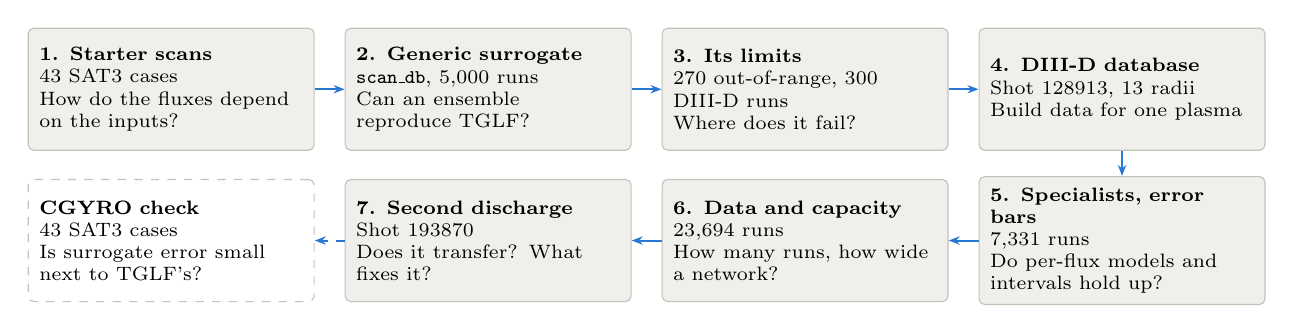
\begin{tikzpicture}[
      stage/.style={draw=FigAxis, rounded corners=2pt, fill=FigBand, align=left,
        text width=3.35cm, minimum height=1.55cm, inner sep=4pt, font=\scriptsize,
        execute at begin node={\hyphenpenalty=10000\exhyphenpenalty=10000}},
      side/.style={stage, fill=white, dashed},
      arr/.style={-{Stealth[length=4pt]}, FigBlue, line width=0.7pt},
      node distance=0.32cm and 0.38cm]
    \node[stage] (s1) {\textbf{1. Starter scans}\\43 SAT3 cases\\How do the fluxes depend on the inputs?};
    \node[stage, right=of s1] (s2) {\textbf{2. Generic surrogate}\\\texttt{scan\_db}, 5,000 runs\\Can an ensemble reproduce TGLF?};
    \node[stage, right=of s2] (s3) {\textbf{3. Its limits}\\270 out-of-range, 300 DIII-D runs\\Where does it fail?};
    \node[stage, right=of s3] (s4) {\textbf{4. DIII-D database}\\Shot 128913, 13 radii\\Build data for one plasma};
    \node[stage, below=of s4] (s5) {\textbf{5. Specialists, error bars}\\7,331 runs\\Do per-flux models and intervals hold up?};
    \node[stage, left=of s5] (s6) {\textbf{6. Data and capacity}\\23,694 runs\\How many runs, how wide a network?};
    \node[stage, left=of s6] (s7) {\textbf{7. Second discharge}\\Shot 193870\\Does it transfer? What fixes it?};
    \node[side, left=of s7] (cg) {\textbf{CGYRO check}\\43 SAT3 cases\\Is surrogate error small next to TGLF's?};
    \draw[arr] (s1) -- (s2);
    \draw[arr] (s2) -- (s3);
    \draw[arr] (s3) -- (s4);
    \draw[arr] (s4) -- (s5);
    \draw[arr] (s5) -- (s6);
    \draw[arr] (s6) -- (s7);
    \draw[arr, dashed] (s7) -- (cg);
  \end{tikzpicture}
  \caption{The seven stages of the project and the CGYRO check. Each box gives the data
    used and the question asked. Stages 1--3 use course datasets; stages 4--7 use TGLF
    runs for DIII-D plasmas, most of which our team generated.}
  \label{fig:pipeline}
\end{figure}

\subsection{Summary of findings}

\begin{itemize}
  \item A five-network ensemble reproduces TGLF on the generic \texttt{scan\_db} scan
        (test $R^2$ 0.96--0.98), but its error grew in 25 of 27 out-of-range tests and it
        overpredicted DIII-D particle flux by a factor of 2.1 (Sections~\ref{sec:res-generic}
        and~\ref{sec:res-limits}).
  \item For DIII-D shot 128913, a separate ensemble for each flux lowered test RMSE by
        6.8\%, 13.2\%, and 22.0\% for $Q_e$, $Q_i$, and $\Gamma_e$ relative to the joint
        baseline. Most of that gain came from training each flux separately; the
        architecture search added 0.7--3.9\% (Section~\ref{sec:res-specialists}).
  \item Validation-calibrated 90\% intervals are accurate where the test data resemble
        the validation data and too narrow between the training radii
        (Section~\ref{sec:res-intervals}).
  \item More runs at the same 13 radii reduce error at those radii, not between them.
        The surrogate's error is already below TGLF's sensitivity to its own numerical
        resolution (Section~\ref{sec:res-data}).
  \item Models trained on one discharge failed on a second one with different geometry.
        Covering the second discharge's inputs and adding the safety factor and magnetic
        shear as inputs restored $R^2$ of 0.58--0.69 on its profile
        (Section~\ref{sec:res-transfer}).
  \item On 43 cases, the surrogate's RMSE against TGLF is 3--8 times smaller than TGLF's
        RMSE against nonlinear CGYRO (Section~\ref{sec:res-cgyro}).
\end{itemize}

Section~\ref{sec:background} reviews related work, Section~\ref{sec:data} describes the
data, Section~\ref{sec:methods} the methods, and Section~\ref{sec:results} the results.
Section~\ref{sec:discussion} discusses what the results imply and their limits.
Appendix~\ref{app:other} reports approaches we explored but did not carry forward, and
Appendix~\ref{app:repro} explains how to reproduce the results.

\section{Background and Related Work}
\label{sec:background}

\paragraph{TGLF and CGYRO.} TGLF \citep{staebler2007} solves a reduced set of
gyrofluid equations for the linear eigenmodes at each binormal wavenumber $k_y$ and turns
their growth rates into fluxes with a saturation rule. The second saturation rule, SAT2
\citep{staebler2021}, was fitted to nonlinear CGYRO simulations, and all TGLF runs in this
report use it. CGYRO \citep{candy2016} solves the nonlinear gyrokinetic equations and is
the reference that saturation rules are built from. \citet{dudding2022} used 43 nonlinear
CGYRO simulations, including hydrogen, deuterium, and tritium versions of the same plasma,
to build a third rule, SAT3, aimed at the isotope dependence of transport. Our starter
dataset is the course's version of those 43 cases, with TGLF-SAT2 runs added.

\paragraph{Neural network surrogates.} \citet{meneghini2017} built neural network
surrogates for TGLF and for the pedestal model EPED1 and used them in coupled core and
pedestal simulations; their TGLF surrogate averaged 32 independently trained networks with
one hidden layer of 60 units. \citet{vandeplassche2020} trained QLKNN, a surrogate for the
quasilinear model QuaLiKiz, and emphasized checking local transport behavior such as
thresholds and trends in addition to aggregate error. \citet{cao2026} built TGLF-WINN,
which supervises the flux contribution at each wavenumber, and tested its design
components one at a time. \citet{zanisi2024} used ensemble disagreement to choose which
QuaLiKiz runs to add to a training set. These works train on databases spanning many
discharges or broad scans; we study what happens when a surrogate is built around one
discharge and then moved to another.

\paragraph{Uncertainty.} Averaging independently initialized networks reduces error
and gives a spread that often grows away from the training data
\citep{lakshminarayanan2017}. That spread is not a calibrated interval by itself. Split
conformal prediction \citep{lei2018} rescales it using held-out residuals so that, for new
cases drawn like the calibration cases, a nominal 90\% interval contains the true value at
least 90\% of the time. The guarantee says nothing about cases unlike the calibration
data, which is where we test it hardest.

\section{Data}
\label{sec:data}

Table~\ref{tab:data} lists every dataset. All fluxes are TGLF-SAT2 outputs in gyro-Bohm
units unless the table says otherwise. Each TGLF case supplies its full input listing and a
flux file with particle, heat, momentum, and energy-exchange blocks for each species; we
read the species from their charges rather than assuming an order.

\paragraph{Course datasets.} The 43 starter cases are controlled scans around a reference
plasma, labeled by 26 letter groups; eight groups have complete hydrogen, deuterium, and
tritium triplets. Some inputs change together; for example, the electron and ion
temperature gradients are equal. \texttt{scan\_db} samples 11 inputs uniformly over fixed
ranges (collision frequency on a logarithmic scale) around one reference case with
circular-like geometry. \texttt{scan\_db\_outside} contains nine groups of 30 cases that
each push one input beyond its \texttt{scan\_db} range, and \texttt{data\_d3d} contains 300
TGLF runs with inputs drawn within the measurement error bars of a DIII-D plasma at
$r/a=0.5$.

\paragraph{DIII-D shot 128913.} The course supplied TGLF inputs for shot 128913 at 13
radii from $r/a=0.20$ to $0.80$. Each of our four members generated 1,000 cases with a
personal random seed. Each case starts from the supplied input at one radius and scales the
electron and ion temperature gradients by independent factors in $[0.6,1.4]$, both density
gradients by one shared factor in $[0.6,1.4]$, the ion-to-electron temperature ratio by a
factor in $[0.75,1.25]$, and the collision frequency by a factor between 0.5 and 2 drawn
uniformly in $\log_{10}$. Geometry and all other settings stay at the supplied values for
that radius. Before generating cases we ran TGLF at the 13 supplied radii and matched all
39 reference fluxes to three significant figures. The merged team table has 3,884 cases,
because one export was missing 116 runs when we merged it; team B's database used the same
recipe. In machine-learning terms, the six model inputs are the five varied quantities and
$r/a$; the geometry inputs change only with radius, so $r/a$ stands in for them.

\begin{table}[tbp]
  \centering
  \footnotesize
  \setlength{\tabcolsep}{4pt}
  \begin{tabular}{@{}p{0.27\linewidth}p{0.15\linewidth}rp{0.28\linewidth}l@{}}
    \toprule
    Dataset & Source & Cases & What varies & Used in \\
    \midrule
    SAT3 starter scans & Course & 43 & One or two inputs per scan; H, D, T & 1, CGYRO \\
    \texttt{scan\_db} & Course & 5,000 & 11 inputs, sampled jointly & 2 \\
    \texttt{scan\_db\_outside} & Course & 270 & One input beyond its range & 3 \\
    \texttt{data\_d3d} & Course & 300 & DIII-D inputs within error bars & 3 \\
    \midrule
    DIII-D \#128913, team A & Our team & 3,884 & 5 local inputs at 13 radii & 4--5 \\
    DIII-D \#128913, team B & Team B & 3,500 & Same recipe & 5 \\
    Cleaned \#128913 pool & Both teams & 23,694 & Same recipe, later release & 6 \\
    Intermediate radii & Course, both & 1,438 & Profile and 5 inputs at 12 radii & 5--6 tests \\
    DIII-D \#193870 & Course, team B & 530 & Profile and 5 inputs at 13 radii & 7 tests \\
    Widened \#128913 database & Sweekrit & 8,000 & Wider ranges, plus $q$ and shear & 7 \\
    \bottomrule
  \end{tabular}
  \caption{Datasets used in this report and the stage that uses each. The starter scans
    come from \citet{dudding2022}. The intermediate radii, $r/a = 0.225, 0.275, \dots, 0.775$,
    lie halfway between the 13 training radii; their 1,438 cases are 12 profile points from
    the course, 240 varied cases from Ryan, and 1,186 from team B. The 530 shot-193870 cases
    are 13 profile points and 517 varied cases. Counts are before quality checks
    (Section~\ref{sec:methods}).}
  \label{tab:data}
\end{table}

The DIII-D database is not a subset of \texttt{scan\_db}. Of the 3,884 team cases, 67\% lie
outside at least one \texttt{scan\_db} design range, mostly because 45\% have a density
gradient $a/L_n$ below the scan's minimum of 1 (Figure~\ref{fig:coverage}). A surrogate
trained on \texttt{scan\_db} must extrapolate for most of this plasma.

\begin{figure}[tbp]
  \centering
  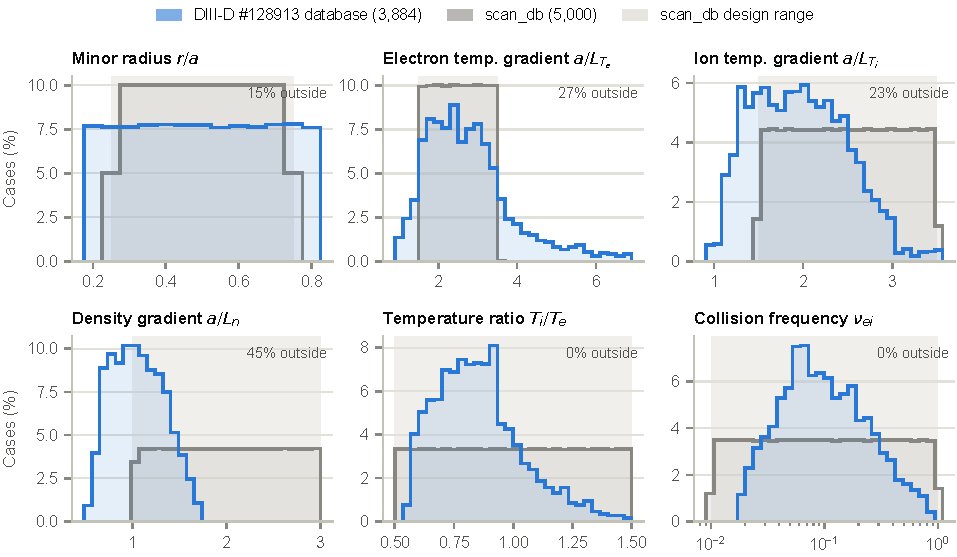
\includegraphics[width=\linewidth]{final_figures/fig_coverage.pdf}
  \caption{Inputs of the 3,884-case DIII-D \#128913 team database (blue) and the 5,000
    \texttt{scan\_db} cases (gray), as the percentage of each dataset in each bin. The
    shaded band is the \texttt{scan\_db} design range, and each panel gives the share of
    DIII-D cases outside it. Collision frequency uses a logarithmic axis.}
  \label{fig:coverage}
\end{figure}

\paragraph{Held-out sets.} The course supplied TGLF inputs and answers at 12 intermediate
radii. Ryan generated 240 varied cases at those radii (20 per radius, seed 180501) and ran
TGLF on them only after the Stage 5 forecasts for them had been frozen. Team B's later
release adds 1,186 varied cases at the same radii, 385 cases rerun at two other TGLF
resolutions, and 517 varied cases and 13 profile points for a second discharge, shot
193870. All eight geometry inputs differ between the two shots at every radius; at
$r/a=0.80$, for example, the safety factor $q$ falls from 2.78 to 1.91 and the
triangularity changes sign. Of the 517 shot-193870 cases, 457 also have at least one of the
five varied inputs outside the shot-128913 factor ranges.

\section{Methods}
\label{sec:methods}

\subsection{Common protocol}
\label{sec:protocol}

Every experiment fixes its train, validation, and test membership before any model is
trained, fits scalers and target transforms on training rows only, and selects
architectures, stopping epochs, and finalists on validation data. Test data are scored only
after those choices are frozen. Ensembles average their members after each member's
inverse target transform, so the average is in gyro-Bohm units. Negative heat flux has no
meaningful logarithm and appears in 4 of the 5,000 \texttt{scan\_db} runs and 53 of the
7,384 Stage 5 DIII-D runs, so those runs are excluded and recorded; negative particle flux is physical and is kept with its sign. We report RMSE in
gyro-Bohm units, $R^2$, and where outputs must share a scale, normalized RMSE (RMSE divided
by the training standard deviation of that flux). Every reported metric compares a
prediction with TGLF unless it names CGYRO.

\subsection{Generic surrogate on \texttt{scan\_db} (Stages 2--3)}
\label{sec:meth-generic}

The \texttt{scan\_db} split is a fixed 70/15/15 random split (seed 42). Four runs with
negative ion heat flux were removed after splitting, leaving 3,496 training, 750 validation,
and 750 test cases. The 11 inputs are the two temperature gradients, the shared density
gradient, the temperature ratio, safety factor, elongation, Shafranov shift, $r/a$, ion
mass, $\log_{10}$ collision frequency, and magnetic shear
$\hat{s} = q' (r/a)^2 / q^2$, reconstructed from the TGLF inputs. The heat fluxes are
modeled as $\log_{10}Q$ and $\Gamma_e$ on its signed scale.

Each network has layers 11--64--64--8--3 with GELU, GELU, and ReLU activations, chosen
among four activation pairs by mean normalized validation RMSE (Appendix~\ref{app:activation}).
Training uses AdamW with weight decay $10^{-4}$, batch size 256, 30 warmup epochs at
learning rate 0.001, then up to 120 epochs at 0.003 with early stopping after 25 epochs
without validation improvement. The ensemble averages five networks (seeds 42--46). We
compared it with a training-mean predictor and a linear model on the same transformed
targets. Appendix~\ref{app:family} compares random forests, gradient boosting, and single
networks on the same data.

For Stage 3 we used a 15-network version of the ensemble (seeds 42--56) with the interval
method of Section~\ref{sec:meth-intervals}, and scored it without retraining on the nine
out-of-range groups and on the 300 \texttt{data\_d3d} runs.

\subsection{DIII-D specialists (Stage 5)}
\label{sec:meth-specialists}

Stage 5 combines both teams' shot-128913 databases. After removing 53 runs with negative
heat flux, 7,331 runs remain, split 70/15/15 (seeds 180510 and 180511) with stratification
by radius: 5,131 training, 1,100 validation, and 1,100 test cases. The six inputs are the
five varied quantities and $r/a$.

The question was whether one network predicting all three fluxes is worse than a separate
network for each. A matched comparison needs the same search effort for both, so the search
ran in stages. It started from four controls: the Stage 2 joint design (64--64--8 hidden units) and the
same design trained separately for each flux. Screening changed one setting at a time
relative to the matching control: width, depth, bottleneck width, activations, and the
transform of each input and target, 114 configurations in all. The best change in each of
four groups (structure, activation, input transform, target transform) was then combined in
all 16 ways for each output mode. The finalists were retrained with three fresh groups of
five seeds and a longer budget of 600 main epochs, and the final choice used the mean
validation score across those repeats. A joint network with about as many parameters as the three specialists
together served as a capacity control. The search trained 194 five-network ensembles,
970 networks in total.

The selected specialists are 64--64--64 units with SiLU and a scaled $\log(1+Q/s)$ target
for $Q_e$; 128--128--8 units with GELU and an untransformed target for $Q_i$; and
64--64--64--8 units with SiLU and a Yeo--Johnson target for $\Gamma_e$. All three dropped
the logarithm of collision frequency. Pooling the three trained repeats of each specialist
gives 15 networks per flux, which we compared with one validation-selected five-network
repeat.

\subsection{Prediction intervals}
\label{sec:meth-intervals}

For an ensemble with mean prediction $\hat{y}$ and member standard deviation $s$, the 90\%
interval is
\begin{equation}
  \hat{y} \pm q \cdot \max\left(s,\ 0.01\,\sigma_{\text{train}}\right),
  \label{eq:interval}
\end{equation}
where $\sigma_{\text{train}}$ is the training standard deviation of that flux and the floor
keeps the interval from collapsing when the members agree. The multiplier $q$ is the
$\lceil 0.9(n+1) \rceil$-th smallest of the $n$ validation ratios
$|y-\hat{y}|/\max(s, 0.01\,\sigma_{\text{train}})$, the split conformal rule of
\citet{lei2018}. Validation cases get their own intervals from five-fold out-of-fold
multipliers, and every other set uses the multiplier fitted on all of validation. For the
240 varied cases at intermediate radii, the forecasts and intervals were written and
hashed before TGLF was run on those inputs, so they are a prospective test. The Stage 3 and
Stage 6 ensembles use the same interval form, with multipliers fitted on their own validation
sets.

\subsection{Data and capacity (Stage 6)}
\label{sec:meth-data}

Team B's later release and our table give 23,694 standard shot-128913 runs after the same
quality checks, split 70/15/15 into 16,586 training, 3,554 validation, and 3,554 test cases.
Every case from the Stage 5 split kept its Stage 5 partition. For each flux we trained a
fresh five-network ensemble of the Stage 5 specialist on nested, radius-stratified subsets
of 1,000, 2,000, 4,000, 8,000, and 16,586 runs, with three independent draws below full size.
At 1,000, 4,000, and 16,586 runs we also trained half and double the hidden width, which
gives 81 ensembles; four-times-wide networks were added later at full size and scored on
validation only. Width comparisons were frozen before the test set was scored.

We scored the 39 original-width ensembles on the test set, on 1,426 varied cases at the
intermediate radii (team B's 1,186 and Ryan's 236 with nonnegative heat flux), and on the 385
cases that TGLF also ran with coarser (2/4) and finer (16/16) settings of its basis-function
count \texttt{NBASIS}; the training data use 12/12. To estimate how many more runs would
halve the error, we fitted $\text{RMSE} \propto n^{-b}$ to the learning curves over all
sizes and over 4,000--16,586 runs.

\subsection{Second discharge (Stage 7)}
\label{sec:meth-transfer}

We scored all 81 Stage 6 ensembles and the pooled Stage 5 specialists, without refitting,
on the 13 shot-193870 profile points and its 517 perturbed cases (Team B's runs at
\texttt{NBASIS} 12/12 with nonnegative heat flux). The handout then asks whether widening
the input ranges and adding the safety factor and magnetic shear as inputs fixes the
transfer. Sweekrit generated 8,000 new TGLF runs around shot 128913 (615 or 616 per radius,
seed 101) with the electron temperature-gradient factor widened to $[0.45, 1.4]$, the
density-gradient factor to $[0.04, 1.4]$ (log-uniform), and the temperature-ratio factor to
$[0.75, 1.35]$, so that shot 193870's values are reachable at every radius. The same runs
also scale $q$ by $[0.65, 1.35]$ and the magnetic shear by $[0.5, 2.5]$. He trained
quantile-regression ensembles (Appendix~\ref{app:quantile}) with eight inputs, the original
six plus $q$ and $q'$, on 7,122 runs with positive heat flux, split 70/15/15, and scored them
on the 13 shot-193870 profile points. The comparison model is the same architecture trained
on the two team databases with six inputs.

\subsection{CGYRO check}
\label{sec:meth-cgyro}

Each of the 43 starter cases has a nonlinear CGYRO simulation and a TGLF-SAT2 run made from
the same inputs. We summed CGYRO's flux output over toroidal modes and both fields
(electrostatic and magnetic) and averaged it over the second half of each run, about
500 normalized time units ($a/c_s$). The standard error of four block means in that window
is a median 2--3\% of the flux. Both codes report gyro-Bohm units with the same reference
mass (deuterium, for all three isotopes), temperature, and magnetic field normalization,
which we checked from each run's CGYRO output and TGLF input. The surrogate is the Stage 2
five-network ensemble, trained on \texttt{scan\_db} only.

\section{Results}
\label{sec:results}

\subsection{Starter scans and the generic surrogate (Stages 1--2)}
\label{sec:res-generic}

The starter scans showed that the three fluxes respond nonlinearly and unevenly to the
inputs and that the outputs move together: $\Gamma_e$ and $Q_e$ correlate at 0.98 across
the 43 cases. Heat fluxes span about two orders of magnitude, which is why we model their
logarithms. On these 43 structured cases, more flexible models did not reliably help, and
the model with the lowest ion-heat error predicted negative heat flux for two cases with
positive TGLF values (Appendix~\ref{app:starter}). From then on we checked signs and
individual failures as well as aggregate error.

On \texttt{scan\_db}, the five-network ensemble reduced test RMSE by 59.6\%, 61.8\%, and
77.2\% for $Q_i$, $Q_e$, and $\Gamma_e$ relative to the linear model (Table~\ref{tab:scandb}).
On the 43 starter cases, which it never saw, it reached $R^2$ of 0.970, 0.997, and 0.988, yet
it matched 25 of 27 temperature-gradient trend directions and predicted the wrong particle
flux sign in two cases. The test cases had been inspected during earlier exploration, so
these scores are not a pristine held-out estimate.

\begin{table}[tbp]
  \centering
  \small
  \begin{tabular}{lrrrrrr}
    \toprule
     & \multicolumn{3}{c}{RMSE (gyro-Bohm)} & \multicolumn{3}{c}{$R^2$} \\
    \cmidrule(lr){2-4}\cmidrule(lr){5-7}
    Model & $Q_i$ & $Q_e$ & $\Gamma_e$ & $Q_i$ & $Q_e$ & $\Gamma_e$ \\
    \midrule
    Training mean & 76.53 & 60.20 & 20.93 & $-0.009$ & $-0.010$ & $-0.011$ \\
    Linear & 38.43 & 29.48 & 14.43 & 0.746 & 0.758 & 0.519 \\
    Five-network ensemble & 15.53 & 11.27 & 3.29 & 0.958 & 0.965 & 0.975 \\
    \bottomrule
  \end{tabular}
  \caption{Generic surrogate on the 750 \texttt{scan\_db} test cases, against TGLF.}
  \label{tab:scandb}
\end{table}

\subsection{Limits of the generic surrogate (Stage 3)}
\label{sec:res-limits}

The 15-network ensemble's intervals covered 91.2\%, 90.1\%, and 91.9\% of the test cases,
close to the nominal 90\%. Outside the training ranges its error rose: RMSE exceeded the
in-range test value in 25 of the 27 group-and-flux combinations, by up to a factor of 10.7
for $\Gamma_e$ when the density gradient left its range (Figure~\ref{fig:limits}a). The two
exceptions were electron heat and particle flux at high collision frequency, where RMSE fell
to 0.39 and 0.50 times its in-range value. Interval coverage on these groups ranged from 60\%
to 100\%.

On the 300 \texttt{data\_d3d} runs the ensemble followed TGLF's trends but sat above it: its
mean prediction was 1.11, 1.12, and 2.06 times TGLF's mean for $Q_i$, $Q_e$, and $\Gamma_e$
(Figure~\ref{fig:limits}b). Every TGLF value fell inside its interval, but the intervals
averaged 3.9 gyro-Bohm units wide for a particle flux whose mean is 0.48, so coverage alone
hid a biased center. These DIII-D inputs lie inside the scan's ranges but in its lowest
quarter for the density gradient (8th percentile), magnetic shear (11th), and safety factor
(23rd). The quantile-regression ensemble of Appendix~\ref{app:quantile} shows the same upward
bias. This result motivated building a database around a DIII-D plasma.

\begin{figure}[tbp]
  \centering
  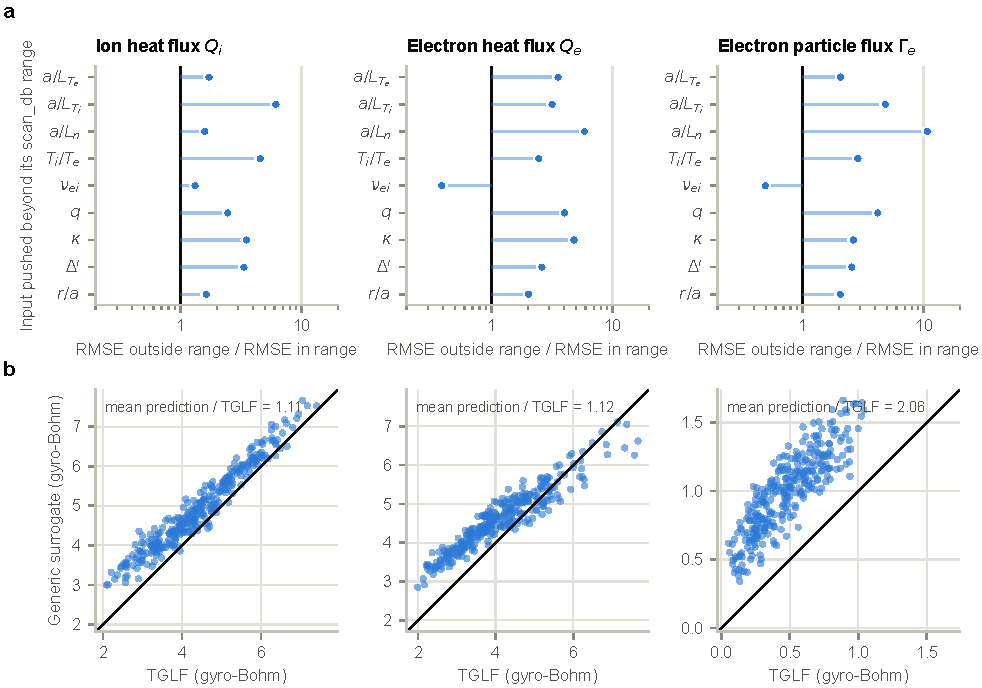
\includegraphics[width=\linewidth]{final_figures/fig_generic_limits.pdf}
  \caption{The generic surrogate away from its training data. (a) RMSE on each group of 30
    cases with one input beyond its \texttt{scan\_db} range, divided by the in-range test
    RMSE; the vertical line marks equal error. (b) Predictions against TGLF for 300 DIII-D
    runs at $r/a=0.5$ with inputs sampled within measurement error bars; the diagonal is
    perfect agreement. Fifteen-network ensemble.}
  \label{fig:limits}
\end{figure}

\subsection{DIII-D specialists (Stages 4--5)}
\label{sec:res-specialists}

The search chose a different architecture for each flux (Section~\ref{sec:meth-specialists}).
Averaged over three independently trained repeats, the specialists' test RMSE was 6.8\%,
13.2\%, and 22.0\% lower than the joint baseline's for $Q_e$, $Q_i$, and $\Gamma_e$
(Figure~\ref{fig:specialists}). Training the unchanged baseline design separately for each
flux already gave most of that improvement: the search added only 3.9\%, 0.7\%, and 2.7\%
beyond it. Tuning a single joint network did not close the gap; its $Q_i$ error rose and
varied widely across repeats. The evidence for specialists over the tuned joint network is
weak: the 95\% case-bootstrap intervals for their RMSE difference include zero for all three
fluxes ($Q_e$: $-2.62$ to $1.46$; $Q_i$: $-1.07$ to $0.22$; $\Gamma_e$: $-0.050$ to $0.005$).
Against the capacity control, only $\Gamma_e$'s interval excludes zero.

\begin{figure}[tbp]
  \centering
  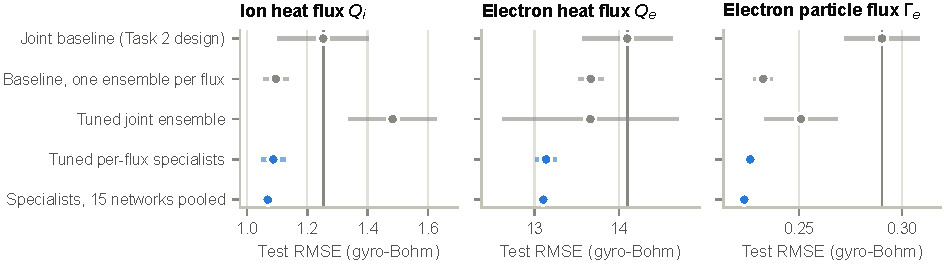
\includegraphics[width=\linewidth]{final_figures/fig_specialists.pdf}
  \caption{Test RMSE on 1,100 held-out shot-128913 cases. Dots are means over three
    independently trained repeats and whiskers one standard deviation across them; the
    vertical line marks the joint baseline. Blue rows are the selected per-flux
    specialists and their 15-network pool.}
  \label{fig:specialists}
\end{figure}

The specialists cost more. The three five-network specialists have 182,895 parameters
against 25,775 for the joint ensemble and took 1.12\,ms rather than 0.38\,ms for one
prediction on our CPU. Lower aggregate error also hid a weakness: the $Q_i$ specialist,
which models the heat flux without a logarithm, predicted negative ion heat flux for 28 of
3,300 test predictions. Pooling all 15 networks per flux changed test RMSE by $+0.1\%$,
$-4.5\%$, and $-1.2\%$ relative to one validation-selected five-network repeat, with 95\%
intervals that include zero, at 2.9 times the inference time.

\subsection{How honest are the error bars? (Stage 5)}
\label{sec:res-intervals}

Table~\ref{tab:intervals} reports the pooled specialists' intervals. On validation and on
the held-out test set, coverage was 90--93\%, as split conformal prediction promises for
cases drawn like the calibration data. On the 240 sealed cases at intermediate radii it fell
to 82--86\%. On those cases the pooled intervals were 36--57\% narrower than the joint
baseline ensemble's, which covered 84--91\%, and the pooled RMSE was 15--25\% lower.

\begin{table}[tbp]
  \centering
  \small
  \begin{tabular}{lrrrrrr}
    \toprule
     & \multicolumn{3}{c}{90\% interval coverage} & \multicolumn{3}{c}{Mean interval width} \\
    \cmidrule(lr){2-4}\cmidrule(lr){5-7}
    Cases & $Q_i$ & $Q_e$ & $\Gamma_e$ & $Q_i$ & $Q_e$ & $\Gamma_e$ \\
    \midrule
    Validation, out of fold (1,100) & 90.3\% & 90.2\% & 90.1\% & 1.63 & 4.02 & 0.33 \\
    Held-out test (1,100) & 91.3\% & 90.9\% & 92.6\% & 1.62 & 3.97 & 0.34 \\
    Intermediate radii, sealed (240) & 84.6\% & 82.1\% & 85.8\% & 1.67 & 4.41 & 0.36 \\
    \bottomrule
  \end{tabular}
  \caption{Coverage and width (gyro-Bohm units) of the pooled specialists' 90\% intervals
    for shot 128913. The 240 intermediate-radius forecasts were frozen before TGLF was run
    on their inputs.}
  \label{tab:intervals}
\end{table}

The Stage 6 full-data ensembles, scored on many more intermediate-radius cases, show where
the intervals fail (Figure~\ref{fig:radius}). At the training radii, coverage was 90\%
overall but fell to 71--79\% for the heat fluxes at $r/a = 0.75$ and $0.80$. Between the
training radii it held at most positions but fell to 39\%, 37\%, and 51\% for $Q_i$, $Q_e$, and
$\Gamma_e$ at $r/a=0.375$, on 120 cases. Between $r/a = 0.375$ and $0.40$, TGLF's nominal
fluxes fall by 53--68\% while each of the six model inputs changes by less than 10\%; the
safety-factor gradient $q'$, which the model does not see, changes by 23\%. A surrogate
trained at the two neighboring radii has no data on where that drop begins, and its members
agree on the wrong answer. Errors relative to flux size are largest at both ends of the
profile, $r/a=0.20$ and $r/a \ge 0.75$.

\begin{figure}[tbp]
  \centering
  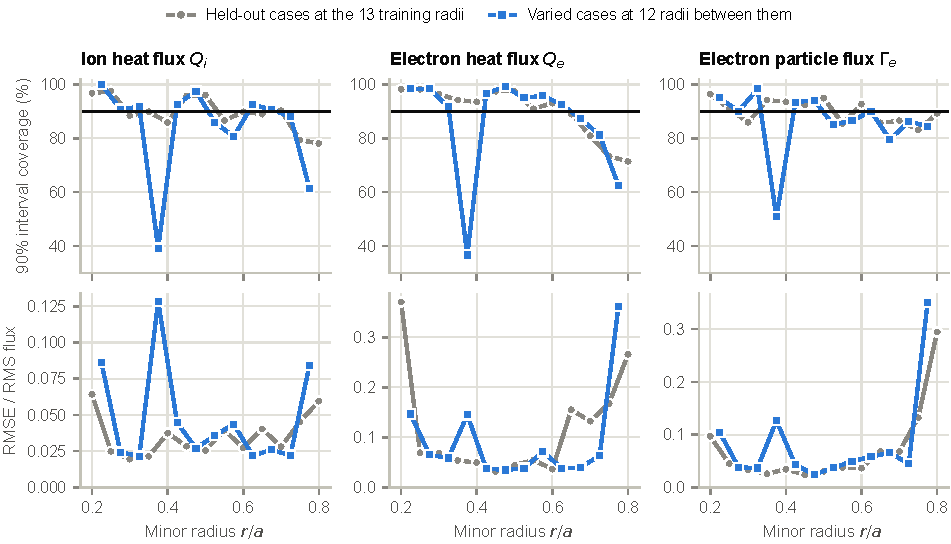
\includegraphics[width=\linewidth]{final_figures/fig_radius.pdf}
  \caption{Interval coverage (top) and RMSE divided by the RMS flux (bottom) by radius for
    the full-data Stage 6 specialists. Gray: held-out cases at the 13 training radii
    (3,554 in all). Blue: varied cases at the 12 radii between them (1,426 in all, about 120
    per radius). The horizontal line marks the nominal 90\%.}
  \label{fig:radius}
\end{figure}

\subsection{How many runs, and how large a network? (Stage 6)}
\label{sec:res-data}

Error was still falling at full size on the training radii (Figure~\ref{fig:learning}). From
8,000 to 16,586 runs, test RMSE fell 4.9\%, 13.6\%, and 14.5\% for $Q_e$, $Q_i$, and
$\Gamma_e$, reaching 10.59, 0.919, and 0.278 gyro-Bohm units. At the intermediate radii the
same doubling changed error by only $-2.0\%$, $-6.3\%$, and $-0.3\%$. The power-law fits put
the cost of halving $Q_i$ test error at 17--20 times the current runs, and of halving $Q_e$
or $\Gamma_e$ test error at more than 100 times; at the intermediate radii the exponents are
0.07--0.11, which no feasible number of runs at the same radii would overcome. These are
order-of-magnitude estimates from five sizes, and at full size the five worst of 3,554
test cases hold 49--74\% of the squared error. More runs at new radii would help more than more runs at the
same 13 radii.

\begin{figure}[tbp]
  \centering
  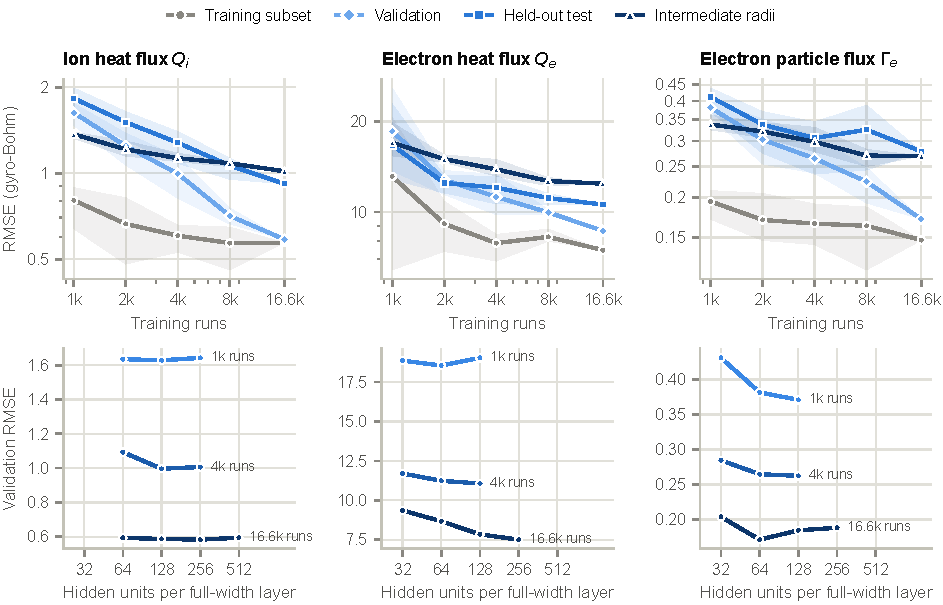
\includegraphics[width=\linewidth]{final_figures/fig_learning.pdf}
  \caption{Top: RMSE against the number of training runs for shot 128913, on logarithmic
    axes. Lines are means over three training draws below full size, and shading spans the
    draws. Bottom: validation RMSE against hidden width at three training sizes. The
    selected specialists use 64 units ($Q_e$, $\Gamma_e$) and 128 units ($Q_i$).}
  \label{fig:learning}
\end{figure}

The width test answers the capacity question. At 1,000 runs, doubling the electron-heat
network lowered training error and raised validation error in two of three draws, the
pattern of overfitting. At full size, $Q_e$ kept improving up to 128 units per layer and
gained nothing measurable from 256 (validation change $-0.34$, 90\% interval $-1.05$ to
$0.37$). $Q_i$ was flat across widths, and $\Gamma_e$ stopped improving above 64 units. About 64--128 units per layer is as
large a network as 16,586 runs support.

Is that error small? Table~\ref{tab:resolution} compares the full-data surrogate with TGLF
itself. Changing TGLF's \texttt{NBASIS} from 12/12 to 16/16 moves its fluxes by a median
5.2--12.0\%, while the surrogate's median difference from the 12/12 result is 2.2--4.7\%.
On these 385 cases the surrogate reproduces TGLF more closely than TGLF reproduces itself at
a finer resolution, so further accuracy against the 12/12 labels has limited physical
meaning.

\begin{table}[tbp]
  \centering
  \small
  \begin{tabular}{lrrr}
    \toprule
    Median relative difference from TGLF at \texttt{NBASIS} 12/12 & $Q_i$ & $Q_e$ & $\Gamma_e$ \\
    \midrule
    Surrogate (full-data specialist) & 2.2\% & 2.4\% & 4.7\% \\
    TGLF at \texttt{NBASIS} 16/16 & 5.2\% & 6.2\% & 12.0\% \\
    TGLF at \texttt{NBASIS} 2/4 & 31.0\% & 23.9\% & 55.8\% \\
    \bottomrule
  \end{tabular}
  \caption{The surrogate's error compared with TGLF's sensitivity to its own resolution,
    on 385 shot-128913 cases run at all three settings.}
  \label{tab:resolution}
\end{table}

\subsection{Transfer to a second discharge (Stage 7)}
\label{sec:res-transfer}

None of the shot-128913 models predicted shot 193870 well (Figure~\ref{fig:transfer}). All
81 Stage 6 ensembles had negative $R^2$ on the 13 profile points, so none followed the
radial shape of the new profile better than its mean. On the 517 perturbed cases, the
full-data models reached $R^2$ of 0.603 for $Q_e$ and $-0.220$ and $-0.418$ for $Q_i$ and
$\Gamma_e$; the pooled Stage 5 specialists scored 0.601, $-0.247$, and $-0.440$. Training on
16 times more shot-128913 runs moved $Q_e$ from 0.45 to 0.60 and left $Q_i$ and $\Gamma_e$
negative. The worst profile errors were at $r/a=0.80$, where $q$ falls from 2.78 to 1.91
between the shots and the triangularity changes sign. Sweekrit's quantile ensembles, a different architecture
trained on the same two team databases, also failed on the profile, with $R^2$ of $-0.99$,
$-1.75$, and $-1.41$.

\begin{figure}[tbp]
  \centering
  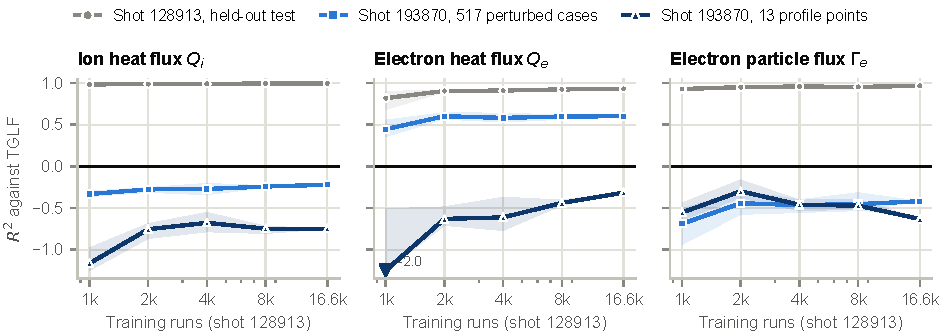
\includegraphics[width=\linewidth]{final_figures/fig_transfer.pdf}
  \caption{$R^2$ against TGLF for the frozen shot-128913 ensembles (original width), by
    number of training runs. Lines are means over training draws and shading spans them.
    The triangle marks a mean below the axis, with its value.}
  \label{fig:transfer}
\end{figure}

The six model inputs cannot represent this change. Radius stands in for geometry within one
discharge, so a model that has learned how flux varies with $r/a$ in shot 128913 applies
that geometry to shot 193870 as well. Retraining on the widened database
(Section~\ref{sec:meth-transfer}) with $q$ and $q'$ as inputs changed the profile result
from failure to useful accuracy (Table~\ref{tab:widened}): $R^2$ rose to 0.60, 0.69, and
0.58, and none of the 13 profile points remained outside the training ranges, compared with
nine before. The new database is harder to fit within its own range (test $R^2$ fell from
0.94, 0.79, and 0.85 to 0.85, 0.66, and 0.81), because it spans a wider domain with two more
inputs. Two cautions apply. The ranges were widened using shot 193870's input values, so
this shows that covering a discharge's inputs fixes the failure, not that the model now
generalizes to unseen discharges. And the comparison uses 13 profile points; the 517
perturbed cases have not been scored with these models.

\begin{table}[tbp]
  \centering
  \small
  \begin{tabular}{lrrrrrr}
    \toprule
     & \multicolumn{3}{c}{$R^2$ on 13 profile points} & \multicolumn{3}{c}{Normalized RMSE} \\
    \cmidrule(lr){2-4}\cmidrule(lr){5-7}
    Training data & $Q_i$ & $Q_e$ & $\Gamma_e$ & $Q_i$ & $Q_e$ & $\Gamma_e$ \\
    \midrule
    Two team databases, 6 inputs & $-0.99$ & $-1.75$ & $-1.41$ & 0.44 & 0.19 & 0.29 \\
    Widened database with $q$, $q'$, 8 inputs & 0.60 & 0.69 & 0.58 & 0.20 & 0.06 & 0.12 \\
    \bottomrule
  \end{tabular}
  \caption{Sweekrit's quantile ensembles on the shot-193870 profile. Normalized RMSE uses
    the training standard deviation of the original team-database model for both rows.
    Median predictions; log heat-flux targets.}
  \label{tab:widened}
\end{table}

\subsection{Surrogate error compared with TGLF's error (CGYRO check)}
\label{sec:res-cgyro}

On the 43 starter cases, the generic surrogate's RMSE against TGLF was 4.2, 1.3, and 1.1
gyro-Bohm units for $Q_i$, $Q_e$, and $\Gamma_e$. TGLF's RMSE against nonlinear CGYRO was
12.7, 10.5, and 4.2, three to eight times larger (Figure~\ref{fig:cgyro}). TGLF-SAT2 sat
below CGYRO in most cases: the median ratio of TGLF to CGYRO flux was 0.89, 0.78, and 0.55.
The averaging uncertainty of the CGYRO fluxes, 2--3\%, is small against these differences.
The surrogate's RMSE against CGYRO (13.3, 10.4, 3.9) is close to TGLF's, because it
reproduces TGLF, gaps included; its slightly lower particle-flux error comes from its
upward bias against TGLF partly cancelling TGLF's downward bias, not from learning CGYRO.

\begin{figure}[tbp]
  \centering
  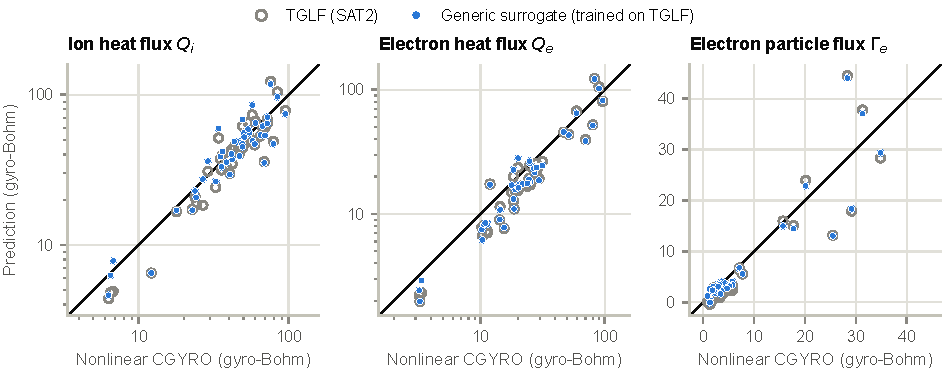
\includegraphics[width=\linewidth]{final_figures/fig_cgyro.pdf}
  \caption{TGLF-SAT2 (gray open circles) and the generic surrogate (blue) against
    time-averaged nonlinear CGYRO fluxes for the 43 starter cases. The diagonal is perfect
    agreement with CGYRO. Heat-flux axes are logarithmic.}
  \label{fig:cgyro}
\end{figure}

\section{Discussion}
\label{sec:discussion}

\paragraph{What a TGLF surrogate needs.} Within one discharge, a modest network trained on
a few thousand runs already reproduces TGLF to within its own numerical sensitivity. The
binding limits are coverage, not capacity. The generic surrogate was biased at a DIII-D
condition near the low end of its scan's ranges; the shot-128913 surrogates lost accuracy between
their training radii, where more runs at the same radii did not help; and they failed on a
second discharge whose geometry they never saw and could not represent. Adding the safety
factor and shear as inputs and sampling the new discharge's ranges restored useful
accuracy. A surrogate meant for more than one plasma therefore needs geometry inputs and
training data that span the geometries and radii it will be used at, and adding runs at
already-covered points buys little.

\paragraph{How far to trust the error bars.} Split conformal intervals did what they promise
for data like their calibration set: 90--93\% coverage on held-out shot-128913 cases. They
promise nothing for shifted data, and they under-covered at intermediate radii and badly at
the sharp radial transition near $r/a=0.375$, where the members agreed on the wrong answer.
At the \texttt{data\_d3d} condition they covered every TGLF value only by being wide around a
biased center. Coverage should be reported with width and with the center's bias, and an
interval calibrated on one discharge does not certify predictions for another.

\paragraph{Limits of this study.} All labels except the CGYRO check are TGLF-SAT2 outputs,
so the results describe agreement with TGLF, not with experiment. The DIII-D work covers two
discharges; the widened database was designed with knowledge of the second discharge's
inputs and was scored on only 13 of its points. Team B's tables lack some TGLF settings,
which we assumed follow the Task 4 recipe. The \texttt{scan\_db} and shot-128913 test sets
had been seen in earlier exploration, so the sealed 240 intermediate-radius cases are the
cleanest held-out test in this report. The CGYRO check uses 43 idealized cases near one
reference plasma, a fixed averaging window, and no estimate of CGYRO's convergence beyond
the block-mean spread.

\paragraph{Next steps.} The CGYRO check shows where the larger error now lies. For these 43
cases, the surrogate's error against TGLF is a fraction of TGLF's error against nonlinear
CGYRO, so further gains in surrogate accuracy against TGLF matter less than correcting TGLF
itself. Our Quarter 2 project will test whether a TGLF surrogate corrected with sparse,
matched nonlinear CGYRO simulations improves agreement with held-out CGYRO cases, evaluating
the correction against CGYRO and the base surrogate against TGLF separately.

\section{Conclusion}
\label{sec:conclusion}

Neural network ensembles reproduce TGLF accurately inside the data they were trained on:
test $R^2$ of 0.96--0.98 on a generic scan, and median errors of 2--5\% on a DIII-D
discharge, below TGLF's own resolution sensitivity. Their failures follow the gaps in their
data: a DIII-D condition near the low end of a generic scan's ranges, radii between the
training radii, and a second discharge with different geometry. Per-flux specialists and pooling
give modest gains whose uncertainty intervals include zero, and validation-calibrated
intervals hold only for data like the validation set. Covering the second discharge's
inputs and adding geometry inputs restored useful accuracy on its profile. For the 43
cases with nonlinear simulations, the surrogate's error is three to eight times smaller
than TGLF's difference from CGYRO.

\makereference

\bibliography{reference}
\bibliographystyle{style/dsc180bibstyle}

\clearpage
\appendix

\section{Other Avenues Explored}
\label{app:other}

These experiments informed the main line of work but did not enter it. Each used its own
split or dataset, so their numbers should not be pooled with the main results.

\subsection{Starter-scan models}
\label{app:starter}

On the 43 starter cases we compared a training-mean baseline, linear models, additive
splines, quadratic terms with interactions, and a random forest, holding out one letter
group at a time so that related isotope cases stayed together (Table~\ref{tab:starter}).
Using the logarithm of collision frequency improved every linear fit. The quadratic model
had the lowest ion-heat error but predicted $-1.34$ and $-20.78$ for two cases with
positive TGLF values of 4.90 and 6.49. The comparison concerns 43 structured cases and does
not show that forests or splines are unsuitable for TGLF in general.

\begin{table}[H]
  \centering
  \small
  \begin{tabular}{lrrr}
    \toprule
    Model & $Q_i$ & $Q_e$ & $\Gamma_e$ \\
    \midrule
    Training mean & 17.022 & 14.830 & 6.127 \\
    Raw linear & 9.570 & 10.215 & 3.520 \\
    Log-collision linear & 8.295 & 7.695 & 2.725 \\
    Additive splines & 17.528 & 11.475 & 3.911 \\
    Quadratic + interactions & 7.965 & 7.253 & 3.210 \\
    Random forest & 16.302 & 11.267 & 3.484 \\
    Log-heat linear & 10.213 & 5.306 & --- \\
    \bottomrule
  \end{tabular}
  \caption{Starter-scan comparison: mean absolute error in gyro-Bohm units across 26
    held-out letter groups, each group weighted equally. The log-heat model was not
    applied to particle flux.}
  \label{tab:starter}
\end{table}

\subsection{Model families on \texttt{scan\_db}}
\label{app:family}

Before building the ensemble, we compared a random forest, XGBoost, and a single MLP, each
trained on raw and log-transformed heat fluxes and tuned by the same cross-validated grid
search, against a ridge baseline. With all 3,496 training cases, the MLP's mean validation
normalized RMSE was 0.233 on raw targets and 0.215 on log targets, against 0.395 and 0.355
for XGBoost and 0.510 and 0.538 for the random forest. The forest trained fastest (0.4--0.9\,s
per fit against 11--13\,s for the MLP) but predicted slowest, about 40--88\,ms per case
against 0.2\,ms for the MLP. On the 43 starter cases the log-target MLP reached normalized
RMSE 0.035 and $R^2$ 0.987, while the ridge baseline and the raw-target forest scored $R^2$ of
$-0.55$ and $-0.07$. These results led us to the network ensemble.

\subsection{Activation search}
\label{app:activation}

With the 11--64--64--8--3 architecture, data, scalers, seeds, and minibatch order held
fixed, we compared four activation pairs on the \texttt{scan\_db} validation set
(Table~\ref{tab:activations}). GELU/ReLU had the lowest mean normalized RMSE, 4.3\% below
GELU/tanh, but its electron-heat error was higher. The learning rate had been tuned for
GELU/tanh, and the alternatives were not retuned.

\begin{table}[H]
  \centering
  \small
  \begin{tabular}{lrrrr}
    \toprule
    Activations & $S$ & $Q_i$ RMSE & $Q_e$ RMSE & $\Gamma_e$ RMSE \\
    \midrule
    GELU / ReLU & 0.1806 & 15.80 & 13.16 & 4.61 \\
    GELU / tanh & 0.1887 & 17.62 & 12.76 & 4.83 \\
    ReLU / tanh & 0.1935 & 18.15 & 12.93 & 4.99 \\
    ReLU / ReLU & 0.2105 & 18.67 & 15.62 & 5.19 \\
    \bottomrule
  \end{tabular}
  \caption{Activation comparison on 750 \texttt{scan\_db} validation cases. The first
    activation applies to both 64-unit layers and the second to the 8-unit layer. $S$ is
    the mean over fluxes of validation RMSE divided by the training standard deviation.}
  \label{tab:activations}
\end{table}

\subsection{Quantile-regression ensembles}
\label{app:quantile}

Sweekrit trained ensembles whose networks output the 5th, 50th, and 95th percentiles of
each flux, using the pinball loss $L_q(e) = \max\{qe, (q-1)e\}$ for error $e = y-\hat{y}$;
the median is the prediction and the outer quantiles form a 90\% interval without a
separate calibration step. Five networks of 11--64--64--8--9 units were averaged. On the
\texttt{scan\_db} test set the medians reached $R^2$ of 0.876, 0.804, and 0.814 for $Q_i$,
$Q_e$, and $\Gamma_e$, and the intervals covered 94.8\%, 93.9\%, and 98.0\%. Interval width
tracked training density: for $Q_i$, average relative width fell as the number of training
cases in a flux bin rose (Spearman $-0.97$). At the \texttt{data\_d3d} condition this
ensemble also sat above TGLF (mean particle flux 1.38 against 0.48) and responded about half
as strongly as TGLF to the density gradient. On the two shot-128913 team databases, with the
six Stage 5 inputs and a split that keeps runs from the same base case together, its test
$R^2$ was 0.940, 0.788, and 0.851, with 94--97\% interval coverage; these are the models in
the first row of Table~\ref{tab:widened}.

\subsection{Gradient-boosted trees with bootstrap intervals}
\label{app:gbdt}

Aryan trained a histogram gradient-boosting regressor \citep{friedman2001,ke2017lightgbm}
for each flux on its own 70/15/15 split of \texttt{scan\_db}, and attached intervals from a
10-member bootstrap ensemble rescaled on validation. On its 750 test cases it reduced RMSE
by 43.5\%, 38.6\%, and 53.6\% for $Q_i$, $Q_e$, and $\Gamma_e$ relative to ridge regression,
with $R^2$ of 0.846, 0.829, and 0.897, and its intervals covered 91.2\%, 87.9\%, and 86.8\%.
Outside the training ranges its error grew by up to a factor of 6.8 while its bootstrap
spread grew far less, because trees extrapolate as constants beyond the last split; coverage
fell to 53\% for $Q_i$ when the ion temperature gradient left its range. Each model trained
in 1--2\,s and predicted in about 12--15\,$\mu$s per case in batches.

\subsection{Further Stage 5 studies}
\label{app:stage5}

Ryan tested four extensions of the selected specialists on the shot-128913 split, each with
a rule for adoption declared before testing. None was carried into Stages 6 and 7.
\begin{itemize}
  \item \emph{Regressor chains} pass one flux's prediction to the next flux's network. The
        best chain (electron heat to ion heat to particle flux) lowered mean validation RMSE
        by 3.0\% and met its validation rule, and it lowered particle-flux test RMSE by 13.9\%,
        but its 95\% interval for the balanced test gain ($-3.8\%$ to $+11.1\%$) included zero.
  \item \emph{Probabilistic chains} pass sampled ion heat flux, rather than its mean, to the
        particle-flux network; this lowered particle-flux RMSE by 2.6\% (interval 1.0\% to
        4.0\%) in a post hoc sensitivity study.
  \item \emph{Wavenumber supervision} added the high-wavenumber part of $Q_e$ as an
        auxiliary target, following \citet{cao2026}. It raised validation RMSE by 24.6\%
        and test RMSE from 13.14 to 13.27.
  \item \emph{Direct weight edits} to the trained specialists did not clear the adoption
        criteria; the best ion-heat edit raised test RMSE by 6.7\%.
\end{itemize}

\section{Reproducing the Results}
\label{app:repro}

The repository's \texttt{README.md} lists the commands for each member's work and
\texttt{DATA.md} explains where to place the course datasets, which are not
redistributed. Ryan's Tasks 4--7 live in \texttt{notebooks/ryan/task4} to
\texttt{task7}; each folder has a README, the scripts, the result tables this report cites,
and a short notebook that displays them. The CGYRO check is in
\texttt{notebooks/ryan/cgyro\_check}. Trained models (about 800\,MB) are not committed, so
reproducing a model result means retraining: several CPU hours for Stages 5 and 6. Every
figure in Section~\ref{sec:results} is drawn by \texttt{quarter\_1\_report/make\_figures.py} from the
committed tables, without retraining. When the code was moved into the repository, each
Stage 4--7 step was rerun against the original saved models and reproduced the original
outputs exactly. Teammates' experiments are in their own folders under \texttt{notebooks/}.

\end{document}
